\documentclass[11pt]{article}

\usepackage{graphicx}
\usepackage{color}
\usepackage{algorithm}
\usepackage{algpseudocode}

\usepackage[T1]{fontenc}
\usepackage[utf8]{inputenc}
\usepackage{indentfirst}

\usepackage[justification=centering]{caption}

\usepackage{amsmath}
\usepackage{amssymb}

\usepackage{multicol}
\usepackage{url}
% \usepackage[hmarginratio=1:1,top=15mm,left=15mm,right=15mm,bottom=15mm,columnsep=15pt]{geometry}
\usepackage{geometry}
\usepackage{siunitx}

\setlength{\parskip}{1em}

\title{HW1 $-$ RNG's with specified distribution}
\author{Enrique Gómez Cruz\\Facultad de Ciencias, Universidad Nacional Autónoma de México.}
\date{}

\begin{document}
\maketitle

\section{Random number generation with specified distribution}
\subsection{Numerical inversion Method}

We have a distribution function $w(x)$ normalized between $x_1$ and $x_2$. The interval $[x_1,x_2]$ is divided in $M$ equal subintervals of size
\begin{equation*}
  I = \frac{x_2-x_1}{M}
\end{equation*}
For each subinterval we apply the recurrence relation in equation~\ref{eqn:numericalInversion} with steps of size $\Delta y$.
\begin{equation}
  x_{i+1} = x_i + \frac{\Delta y}{w(x_i)}
  \label{eqn:numericalInversion}
\end{equation}
The step size should be less than $I$. For example, we chose
\begin{equation*}
  \Delta y = \frac{I}{M} = \frac{x_2-x_1}{M^2}
\end{equation*}

\begin{algorithm}
 \caption{Numerical inversion method} 
 \label{inversionAlgorithm}
 \begin{algorithmic}[1]
 \State $x\leftarrow x_1$ \Comment{Start at lower bound}
 \For{each index $k\in[1,2,\dots,M]$} \Comment{$M$ subintervals, each with upper bound $I k$}
 \State $x \leftarrow x + \Delta y/w(x)$
 \While{$x \le I k$} \Comment{Until end of interval is reached}
 \State X.push($x$)
 \State $x \leftarrow x + \Delta y/w(x)$
 \EndWhile
 \State $x \leftarrow I k$ \Comment{Start at beginning of next interval}
 \EndFor
 \end{algorithmic}
\end{algorithm}

As an example, take $w(x)$ to be as in equation~\ref{eqn:pdf}, normalized in the interval $[0,\pi]$.
\begin{equation}
  w(x)=\frac{\sin^2(2x) + \cos^2(x)}{\pi}
  \label{eqn:pdf}
\end{equation}

We use algorithm~\ref{inversionAlgorithm} to get the random variable $X$ with distribution $w$, and then we use $X$ to calculate the histogram and cdf of $w$. The outputs produced with gnuplot are shown in figures~\ref{fig:inversion-sincos100} and~\ref{fig:inversion-sincos1000}. The former use 100 intervals and the latter 1000 intervals.
\begin{figure}[H]
  \centering

  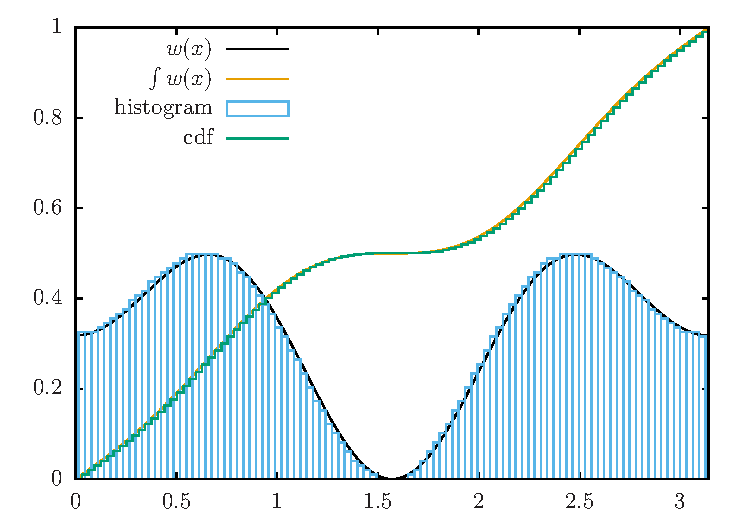
\includegraphics[width=.6\linewidth]{inversion-sincos100}
  \caption{Inversion method with 100 equal intervals.}
\label{fig:inversion-sincos100}

  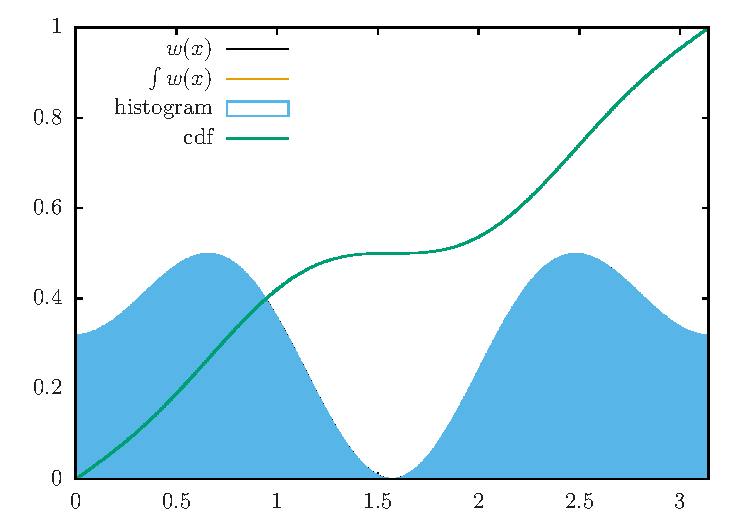
\includegraphics[width=.6\linewidth]{inversion-sincos1000}
  \caption{Inversion method with 1000 equal intervals.}
\label{fig:inversion-sincos1000}
\end{figure}


Initially, the method applied equation~\ref{inversionAlgorithm} to the whole interval $[x_1,x_2]$ instead of applying it to individual subintervals of the form $[x_i-\epsilon,x_i+\epsilon]$. This made the method useless because when $w(x)\rightarrow 0$, $x$ jumped out of the region of integration. Dividing the region of integration into $M$ equally spaced intervals and applying equation~\ref{inversionAlgorithm} in each interval made the method work.

Now, looking at figures~\ref{fig:inversion-sincos100} and~\ref{fig:inversion-sincos1000} we can see that dividing into a bigger number of subintervals, $M$, we get a better approximation of the density function.

\subsection{von Neumann rejection method}
This method uses one distribution $w(x)$ and one function $w'(x)$. Function $w'(x)$ is an upper bound of $w(x)$ for all $x$.

The region of integration is divided in $M$ subintervals of size
\begin{equation*}
  \Delta x = \frac{x_2-x_1}{M}
\end{equation*}

For each value $x = x_1 + i\Delta x$ $(i=0,1,\dots,M)$  a random uniform value, $\eta$, is generated. If $\eta$ is less than the probability of acceptance, $w(x)/w'(x)$, then the value $x$ is accepted.
\begin{algorithm}
 \caption{Rejection/Acceptance method} 
 \label{rejectionAlgorithm}
 \begin{algorithmic}[1]
 \State $x\leftarrow x_1$
 \While{$x\le x_2$}
 \State $\eta\leftarrow \text{uniform random between 0 and 1}$
 \If{$\eta \le w(x)/w'(x)$}
 \State X.push($x$)
 \EndIf
 \State $x \leftarrow x + \Delta x$
 \EndWhile
 \end{algorithmic}
\end{algorithm}

Once again equation~\ref{eqn:pdf} is used as the example. Figures~\ref{fig:rejection-sincos100} and~\ref{fig:rejection-sincos1000} show the outputs produced with gnuplot.
\begin{figure}[H]
  \centering

  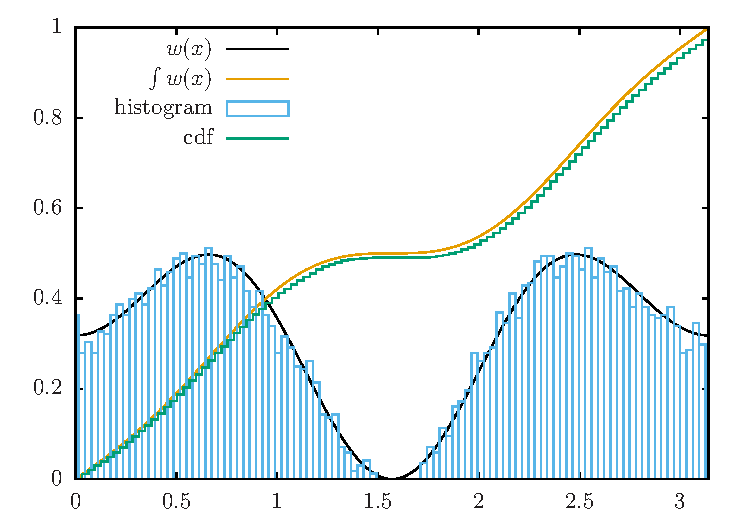
\includegraphics[width=.6\linewidth]{rejection-sincos100}
  \caption{Rejection method with 100 equal intervals.}
\label{fig:rejection-sincos100}

  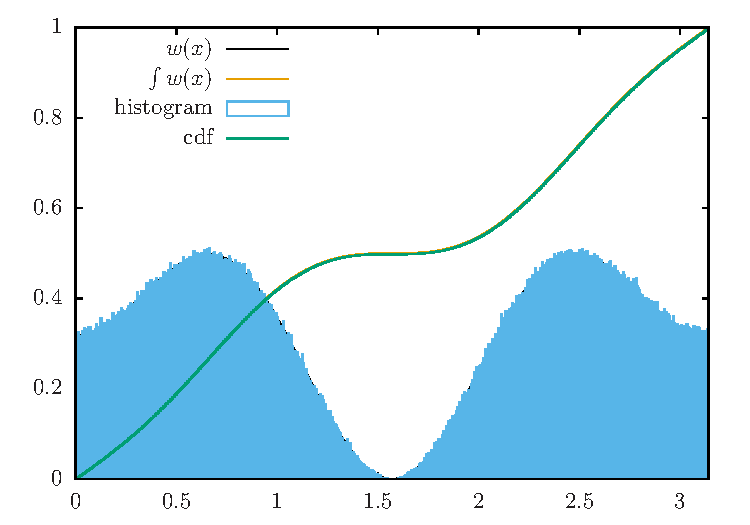
\includegraphics[width=.6\linewidth]{rejection-sincos1000}
  \caption{Rejection method with 1000 equal intervals.}
\label{fig:rejection-sincos1000}
\end{figure}

There's a clear difference between the rejection method and the inversion method. The inversion method makes a more precise approxi mation of the density function because it is not using a random uniform value that produces noise. Nonetheless, both methods achieve almost the same looking plots with the same partition of the region of integration.

\subsection{Metropolis method}

The region of integration, $[x_1,x_2]$, was divided in $M$ equally spaced subintervals of size $\Delta M$. Each point in the partition is given by $x_1 + i \Delta M$ where $i=0,1,\dots,M$. There are $M+1$ walkers each positioned in a different point of the parition. Every walker is going to sample, in $s$ steps, a percentage of the region of integration by making random steps (using $\eta_1$, a random uniform number between 0 and 1) of size $\delta$.

\begin{algorithm}
 \caption{Metropolis method} 
 \label{metropolisAlgorithm}
 \begin{algorithmic}[1]
 \For{each index $i\in[0,1,\dots,M]$}
 \State{$X.push(x_1 + i \Delta M$)}
 \For{each index $j\in[1,2,\dots,s]$}
 \State $X_n\leftarrow X.back()$ \Comment{Get last item in $X$ and save it as $X_n$}
 \State $X_t\leftarrow X_n + (2\eta_1 - 1)\delta$\Comment{Trial step}
 \If{$w(X_t)/w(X_n)>\eta_2$}\Comment{$\eta_2$ random uniform number in $[0,1]$}
 \State $X.push(X_t)$

 \EndIf
 \EndFor
 \EndFor
 \end{algorithmic}
\end{algorithm}

This was the heaviest method of the three, taking 20 seconds longer to output the plot with 1000 walkers. As the density of the walkers become greater the approximation also becomes better. And also as the walk becomes larger the approximation to the distribution function becomes better. It was found experimentally that the step size, $\delta$, was better off being
\begin{equation*}
  \delta = \Delta M
\end{equation*}

\begin{figure}[H]
  \centering

  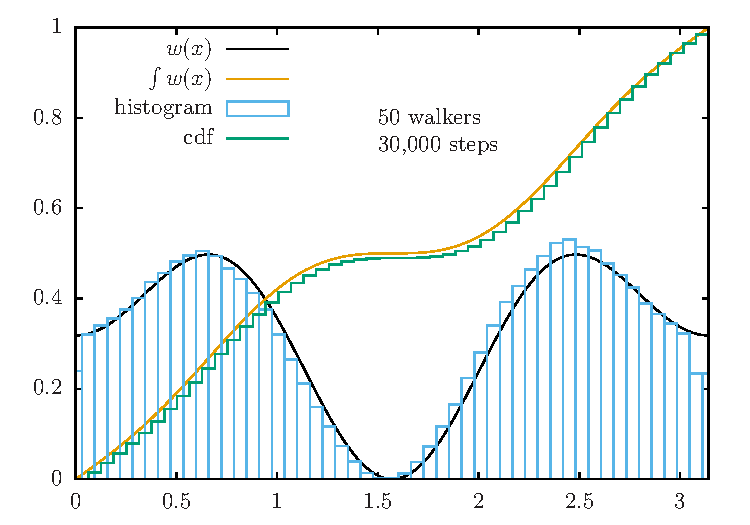
\includegraphics[width=.6\linewidth]{metropolis-sincos50}
  \caption{Metopolis method with 50 walkers and 30,000 steps.}
\label{fig:metropolis-sincos50}
  \centering
  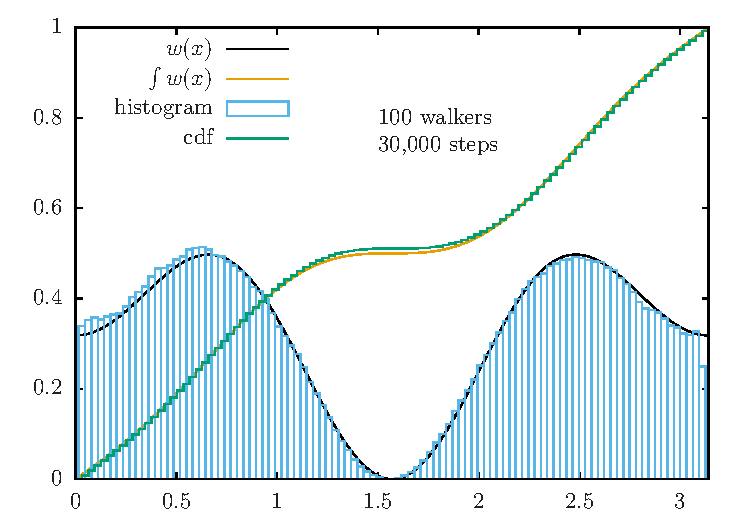
\includegraphics[width=.6\linewidth]{metropolis-sincos100}
  \caption{Metopolis method with 100 walkers and 30,000 steps.}
\label{fig:metropolis-sincos100}
\end{figure}

As the walk size tends to infinity the metropolis algorithm gets to equilibrium. This process of equilibrium is plotted in figures~\ref{fig:metropolisEquilibrium-sincos50} and~\ref{fig:metropolisEquilibrium-sincos100}. It can be seen that the bigger the number of walkers becomes, the bigger the walk size must be. This is seen due to the fact that 50 walkers with a walk size of 1000 is better than 100 walkers with a walk size of 1000.

\begin{figure}[H]
  \centering

  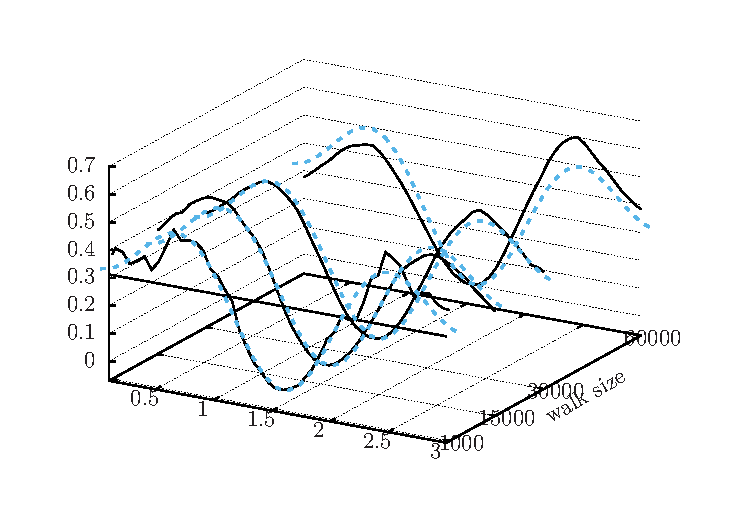
\includegraphics[width=.8\linewidth]{metropolisEquilibrium-sincos50}
  \caption{Equilibrium process in metropolis algorithm with 50 walkers and walk sizes of 1, 1000, 15000, 30000, 60000 steps.}
\label{fig:metropolisEquilibrium-sincos50}

  \centering
  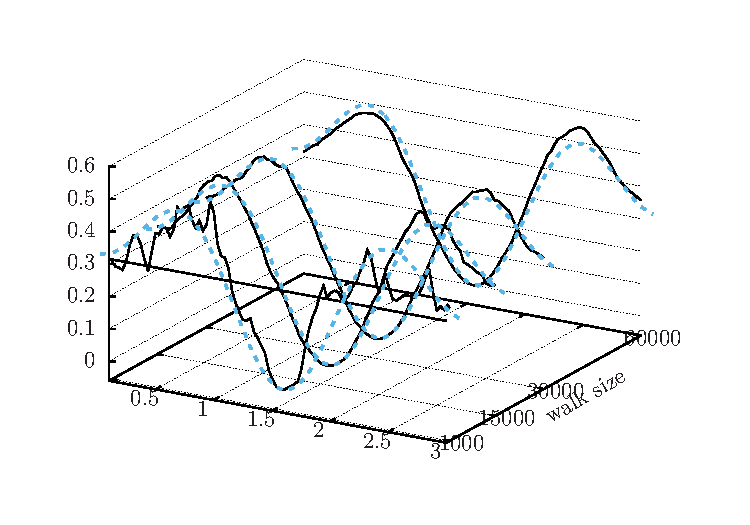
\includegraphics[width=.8\linewidth]{metropolisEquilibrium-sincos100}
  \caption{Equilibrium process in metropolis algorithm with 100 walkers and walk sizes of 1, 1000, 15000, 30000 and 60000 steps.}
\label{fig:metropolisEquilibrium-sincos100}
\end{figure}

\subsection{A Gaussian distribution}
\begin{equation*}
  w(x) = \frac{1}{\sqrt{\pi}}e^{-x^2}
\end{equation*}

This distribution is normalized in the interval of $[-\infty,\infty]$ but since it quickly goes to zero we don't need to sample the whole interval.
\vfill
\begin{figure}[H]
  \centering

  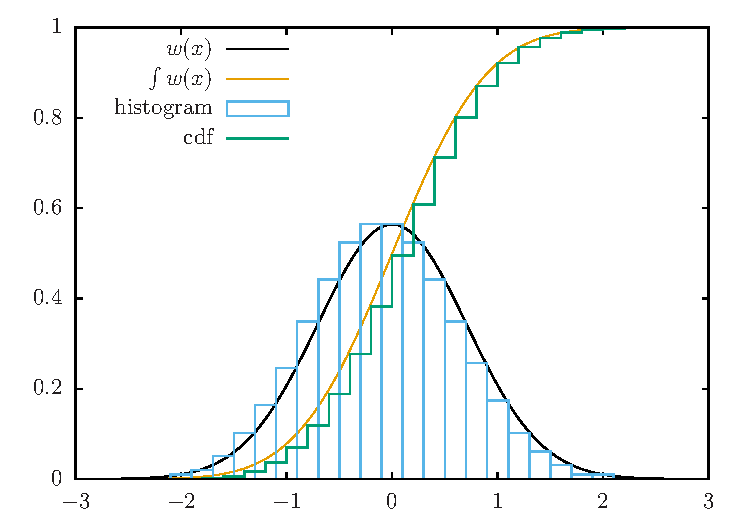
\includegraphics[width=.6\linewidth]{inversion-gaussian100}
  \caption{Inversion method with 100 equal intervals.}
\label{fig:inversion-gaussian100}

  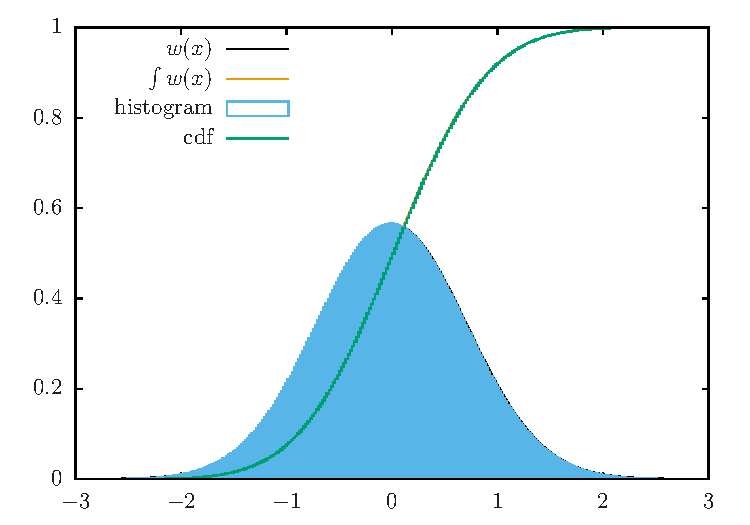
\includegraphics[width=.6\linewidth]{inversion-gaussian1000}
  \caption{Inversion method with 1000 equal intervals.}
\label{fig:inversion-gaussian1000}
\end{figure}

\begin{figure}[H]
  \centering
  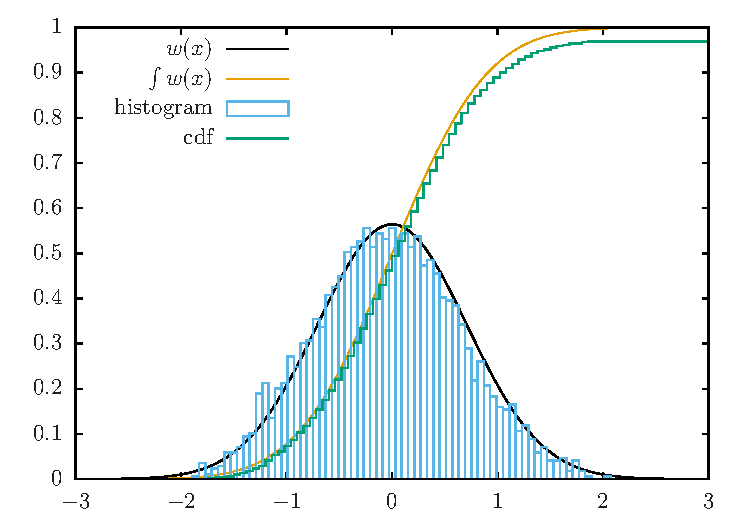
\includegraphics[width=.6\linewidth]{rejection-gaussian100}
  \caption{Rejection method with 100 equal intervals.}
\label{fig:rejection-gaussian100}

  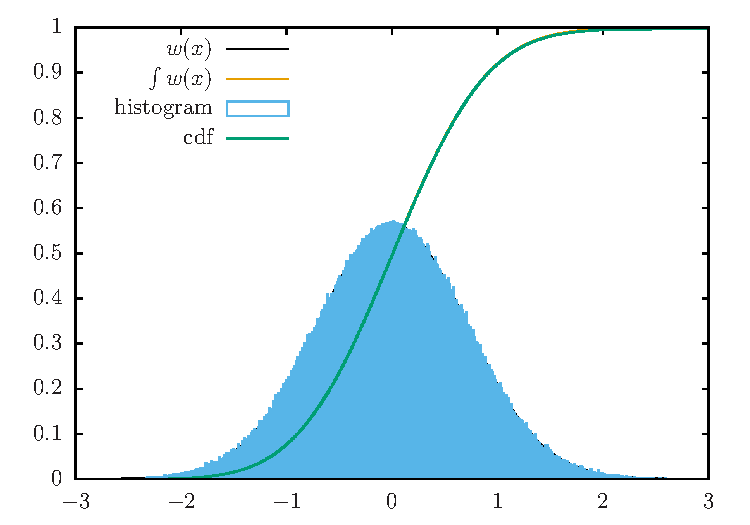
\includegraphics[width=.6\linewidth]{rejection-gaussian1000}
  \caption{Rejection method with 1000 equal intervals.}
\label{fig:rejection-gaussian1000}
\end{figure}

\begin{figure}[H]
  \centering
  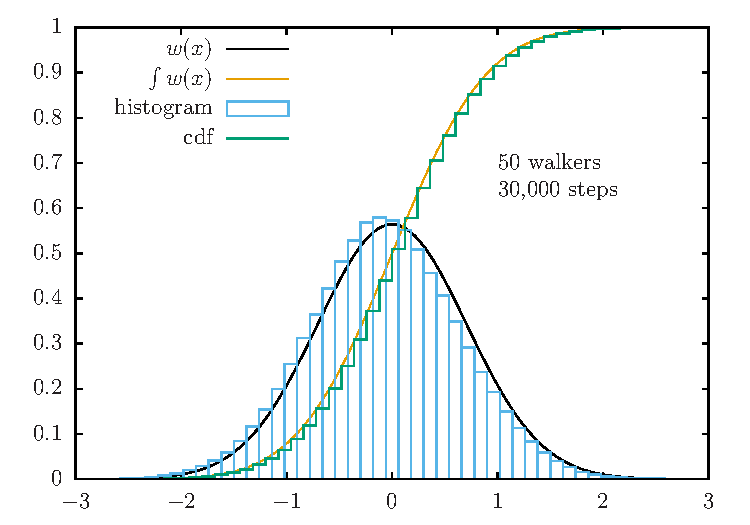
\includegraphics[width=.6\linewidth]{metropolis-gaussian50}
  \caption{Metropolis method with 50 walkers and 30,000 steps.}
\label{fig:metropolis-gaussian50}

  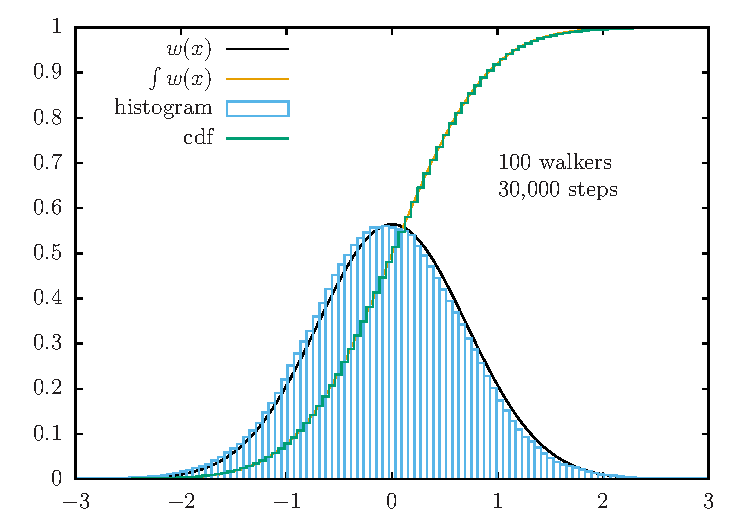
\includegraphics[width=.6\linewidth]{metropolis-gaussian100}
  \caption{Metropolis method with 100 walkers and 30,000 steps.}
\label{fig:metropolis-gaussian100}
\end{figure}

The equilibrium process of the metropolis algorithm is shown in the next figures.
\begin{figure}[H]
  \centering
  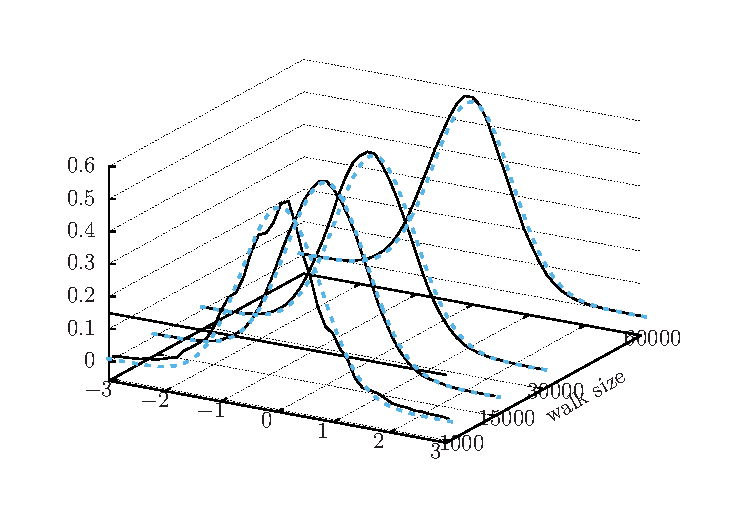
\includegraphics[width=.8\linewidth]{metropolisEquilibrium-gaussian50}
  \caption{Equilibrium process in metropolis algorithm with 50 walkers and walk sizes of 1, 1000, 15000, 30000, 60000 steps.}
\label{fig:metropolisEquilibrium-gaussian50}

  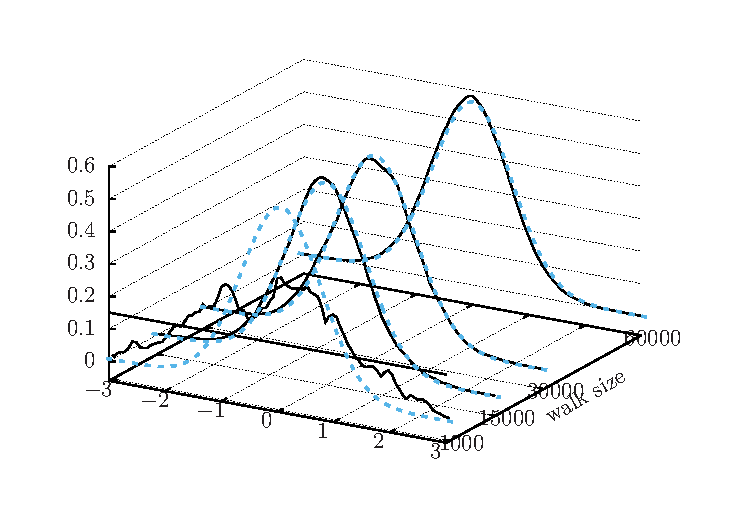
\includegraphics[width=.8\linewidth]{metropolisEquilibrium-gaussian100}
  \caption{Equilibrium process in metropolis algorithm with 100 walkers and walk sizes of 1, 1000, 15000, 30000 and 60000 steps.}
\label{fig:metropolisEquilibrium-gaussian100}
\end{figure}
\end{document}
